\chapter{Introduction}
%\label{chap:intro}
Within this chapter, the reader receive an outline of the general context which surrounds this thesis. Starting with the research motivation and the target goal, a summary of the thesis' structure follows. And finally, an overview of related work is presented.  


\section{Motivation}
Besides the obvious application of WE in the search engine, there are also so-called vertical web services where WE is widely used too. Such websites allow to explore and work with the information on a specific topic. Such services usually do not produce the content by themselves, and rather they automatically collect the data from various sources, processes this data in some way and present to the user in the appealing form. Such services also called \textit{aggregators}. A broad list of aggregators topics includes news, retail other advertisements, reviews, flight tickets, videos and pictures, recipes, social networks and many other. The list is very extensive, virtually for any subject discussed and presented on the Internet there are aggregators exist which try to grasp all other sources into one. \\

Aggregators are usually very popular because they provide the user with the big database, rich functionality, flexibility and instant updates, what helps a user to save time. Due to popularity of aggregator the 'original' content maker is becoming popular too and therefore the content maker has resources to produce new interesting content. The other side of this practice is traffic reduction on the original content maker websites. It happens for example if the aggregator is unfair and doesn't show the source of information. \\

The relationship between aggregators and original source makers today reminds the problem of chicken and egg. That's why search engines are very accurate with automatic extraction at the moment of showing the result for the search query. If Google shows you the correct answer right when you type the question, the website with this particular answer where Google took the information from will lose the user. Since this site loses the user, it also loses monetizing and resources to produce the 'correct answers' in future; hence Google will lose the sources of correct answers. That's the reason why WE among Internet industry players is a controversial topic.\\

In the research area, WE is typically used in the tasks related to natural language processing and text mining. The reason for this is that the web page content is the semi-structured text mixed with the HTML markdown. Many research project centered around the analysis of various news sources as news articles, tweets, social networks, etc. Some of the possible tasks are sentiment analysis of news, topic recognition, summarization. \\

Some projects aim to build the system which collects huge amount of data, extract entities from them, determine relationships between them and my answer on human-language question (IBM Watson \cite{IBMAlchemy}, Calais by Reuters \cite{Calais}, Wolfram Language \cite{Wolfram}).\\      

The extraction of data from the web page is closely linked with the Document Object Model (DOM) processing and implies the understanding of the web page structure from the 'browser point of view'. \\

In this way, WE is becoming a quite interesting, actual and challenging task. It includes both the technical background for the data retrieving and manipulation as well as theoretical background for the reasonable model building. This thesis includes all necessary parts of this task.



In this thesis, we won't solve the problem of identifying if the event announcement is placed on the web page since it is the task from Information Retrieval field. We assume that the page already has an event and we want to find and extract the structured information about it (i.e. extract four items above). On the picture \ref{fig:webevent} you can see a typical example of the page where four main event components are circled in red.\\

We consider \textit{the webpage} as the rendered page where primary JavaScript already executed (it may be executed in future if the user interacts with a page). Such page has several important components: DOM tree, corresponding CSS, HTML code, resources (e.g. images) and rendered picture which the browser displays us. \\

For a webpage, we will collect all web elements from a DOM tree, and four of them would be components we need to extract. We will collect more than two hundreds features for every web element and build the model which distinguishes an event components from all other elements. In our problem we will consider four one-vs-all classifiers where each of them will detect associated event component. 

\begin{figure}[h]
\begin{center}
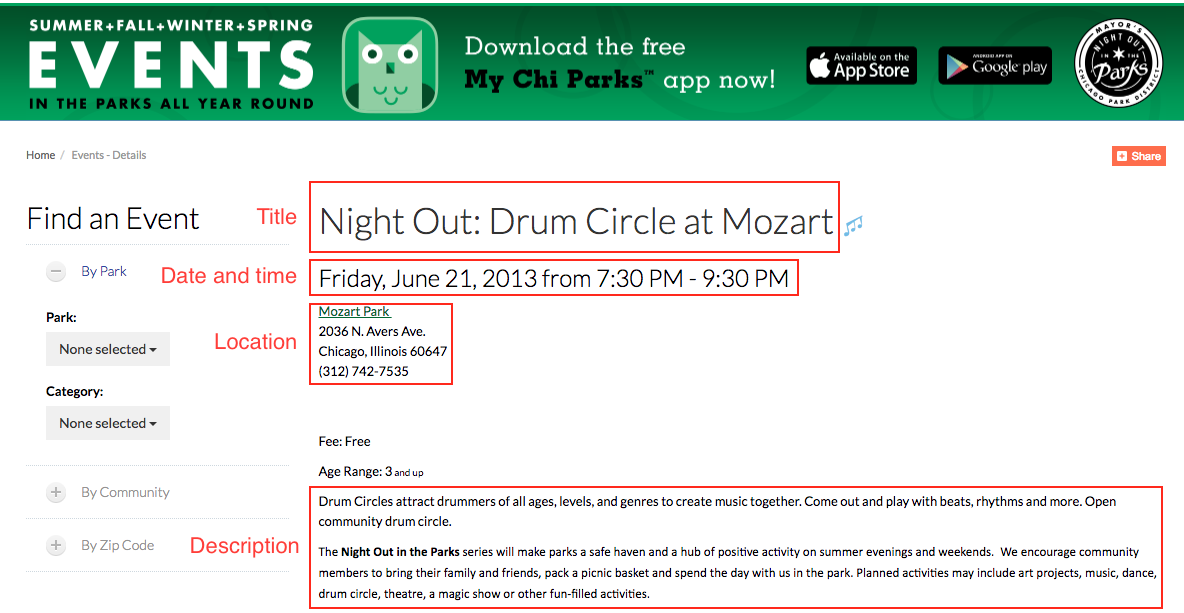
\includegraphics[height=7cm]{figures01/event_example}
\caption{An example of the social event on a webpage}
\label{fig:webevent}
\end{center}
\end{figure}


\section{Thesis Outline}
The thesis consists of 8 chapters, \nameref{appendix} and \nameref{chap:cd}. The current chapter briefly describes the idea of the thesis and motivation for the task of web extraction. Chapter \ref{chap:background} covers necessary web concepts for this work: webpage, DOM, XPath, Microdata semantic markup, etc. Chapter \ref{chap:webextr} refers to an overview of state of the art Web Extraction techniques, overview of complementary problems from IE and related work. In Chapter \ref{chap:design} we explain the structure of our system together with the description of its main components. The method which we propose for the collecting of the training dataset will be discussed in details in Chapter \ref{chap:datacollect}. \\

Last three chapters are devoted to an iterative technical process of the dataset analysis. In Chapter \ref{chap:clean} we will do several cleaning procedures in order to make the dataset reliable. In Chapter \ref{chap:dataexplore} we show the visualization and precise analysis of the extracted features and its relationships. In Chapter \ref{chap:model} we will build  and evaluate several classification models. \nameref{chap:conclusion} will sum up our most valuable contributions and propose ideas for further work.
